\documentclass{beamer}

% Choose a cleaner, more minimalistic theme
\usetheme{metropolis}
\usecolortheme{default}

\usepackage{graphicx}

\title{Making GitHub Pull Requests}
\subtitle{A Guide for Beginners}
\author{Alan Matthew \\ {\small \texttt{@yokurang on GitHub}}}
\date{\today}

\begin{document}

\frame{\titlepage}

\begin{frame}{Comment Your Code}
    When you write your code and need assistance, ensure your comments clarify the issue.
    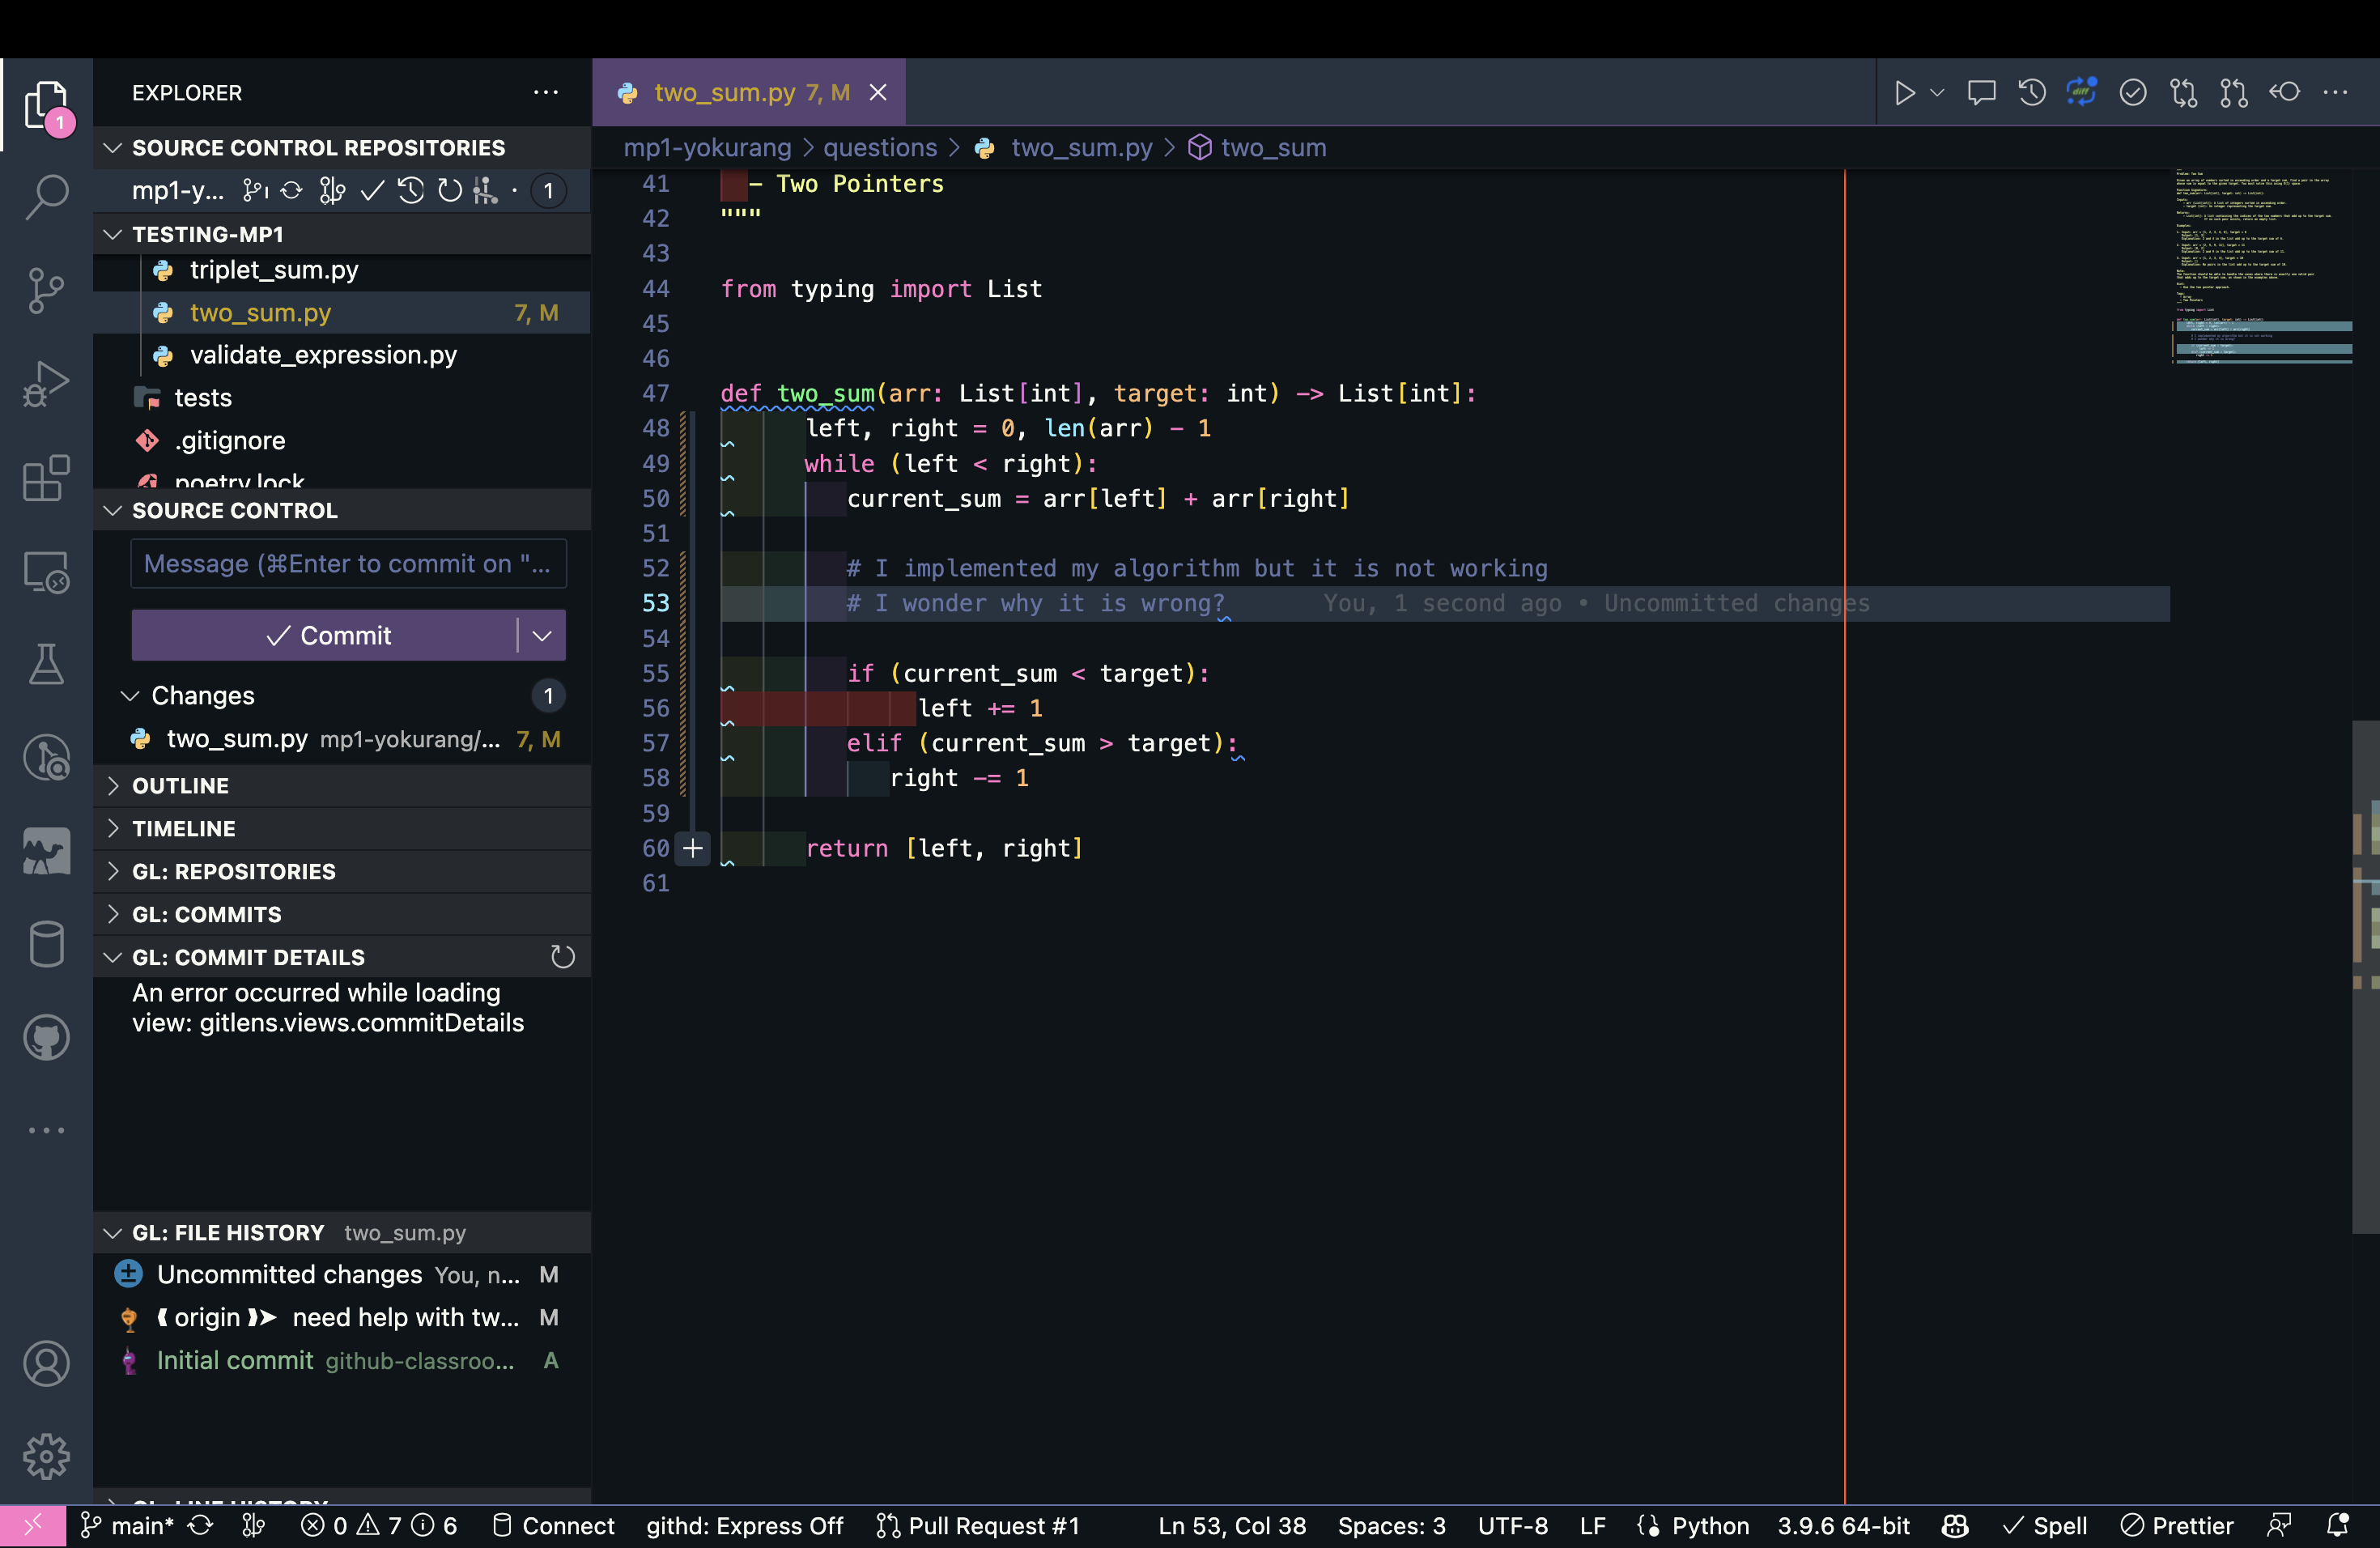
\includegraphics[width=\textwidth,height=0.6\textheight,keepaspectratio]{assets/write-some-code.png}
\end{frame}

\begin{frame}{Create a New Branch}
    Use these commands to create a new branch, stage, commit, and push:
    \begin{itemize}
        \item \texttt{git checkout -b <branch-name>}
        \item \texttt{git add .}
        \item \texttt{git commit -m "Your Message"}
        \item \texttt{git push -u origin <branch-name>}
    \end{itemize}
    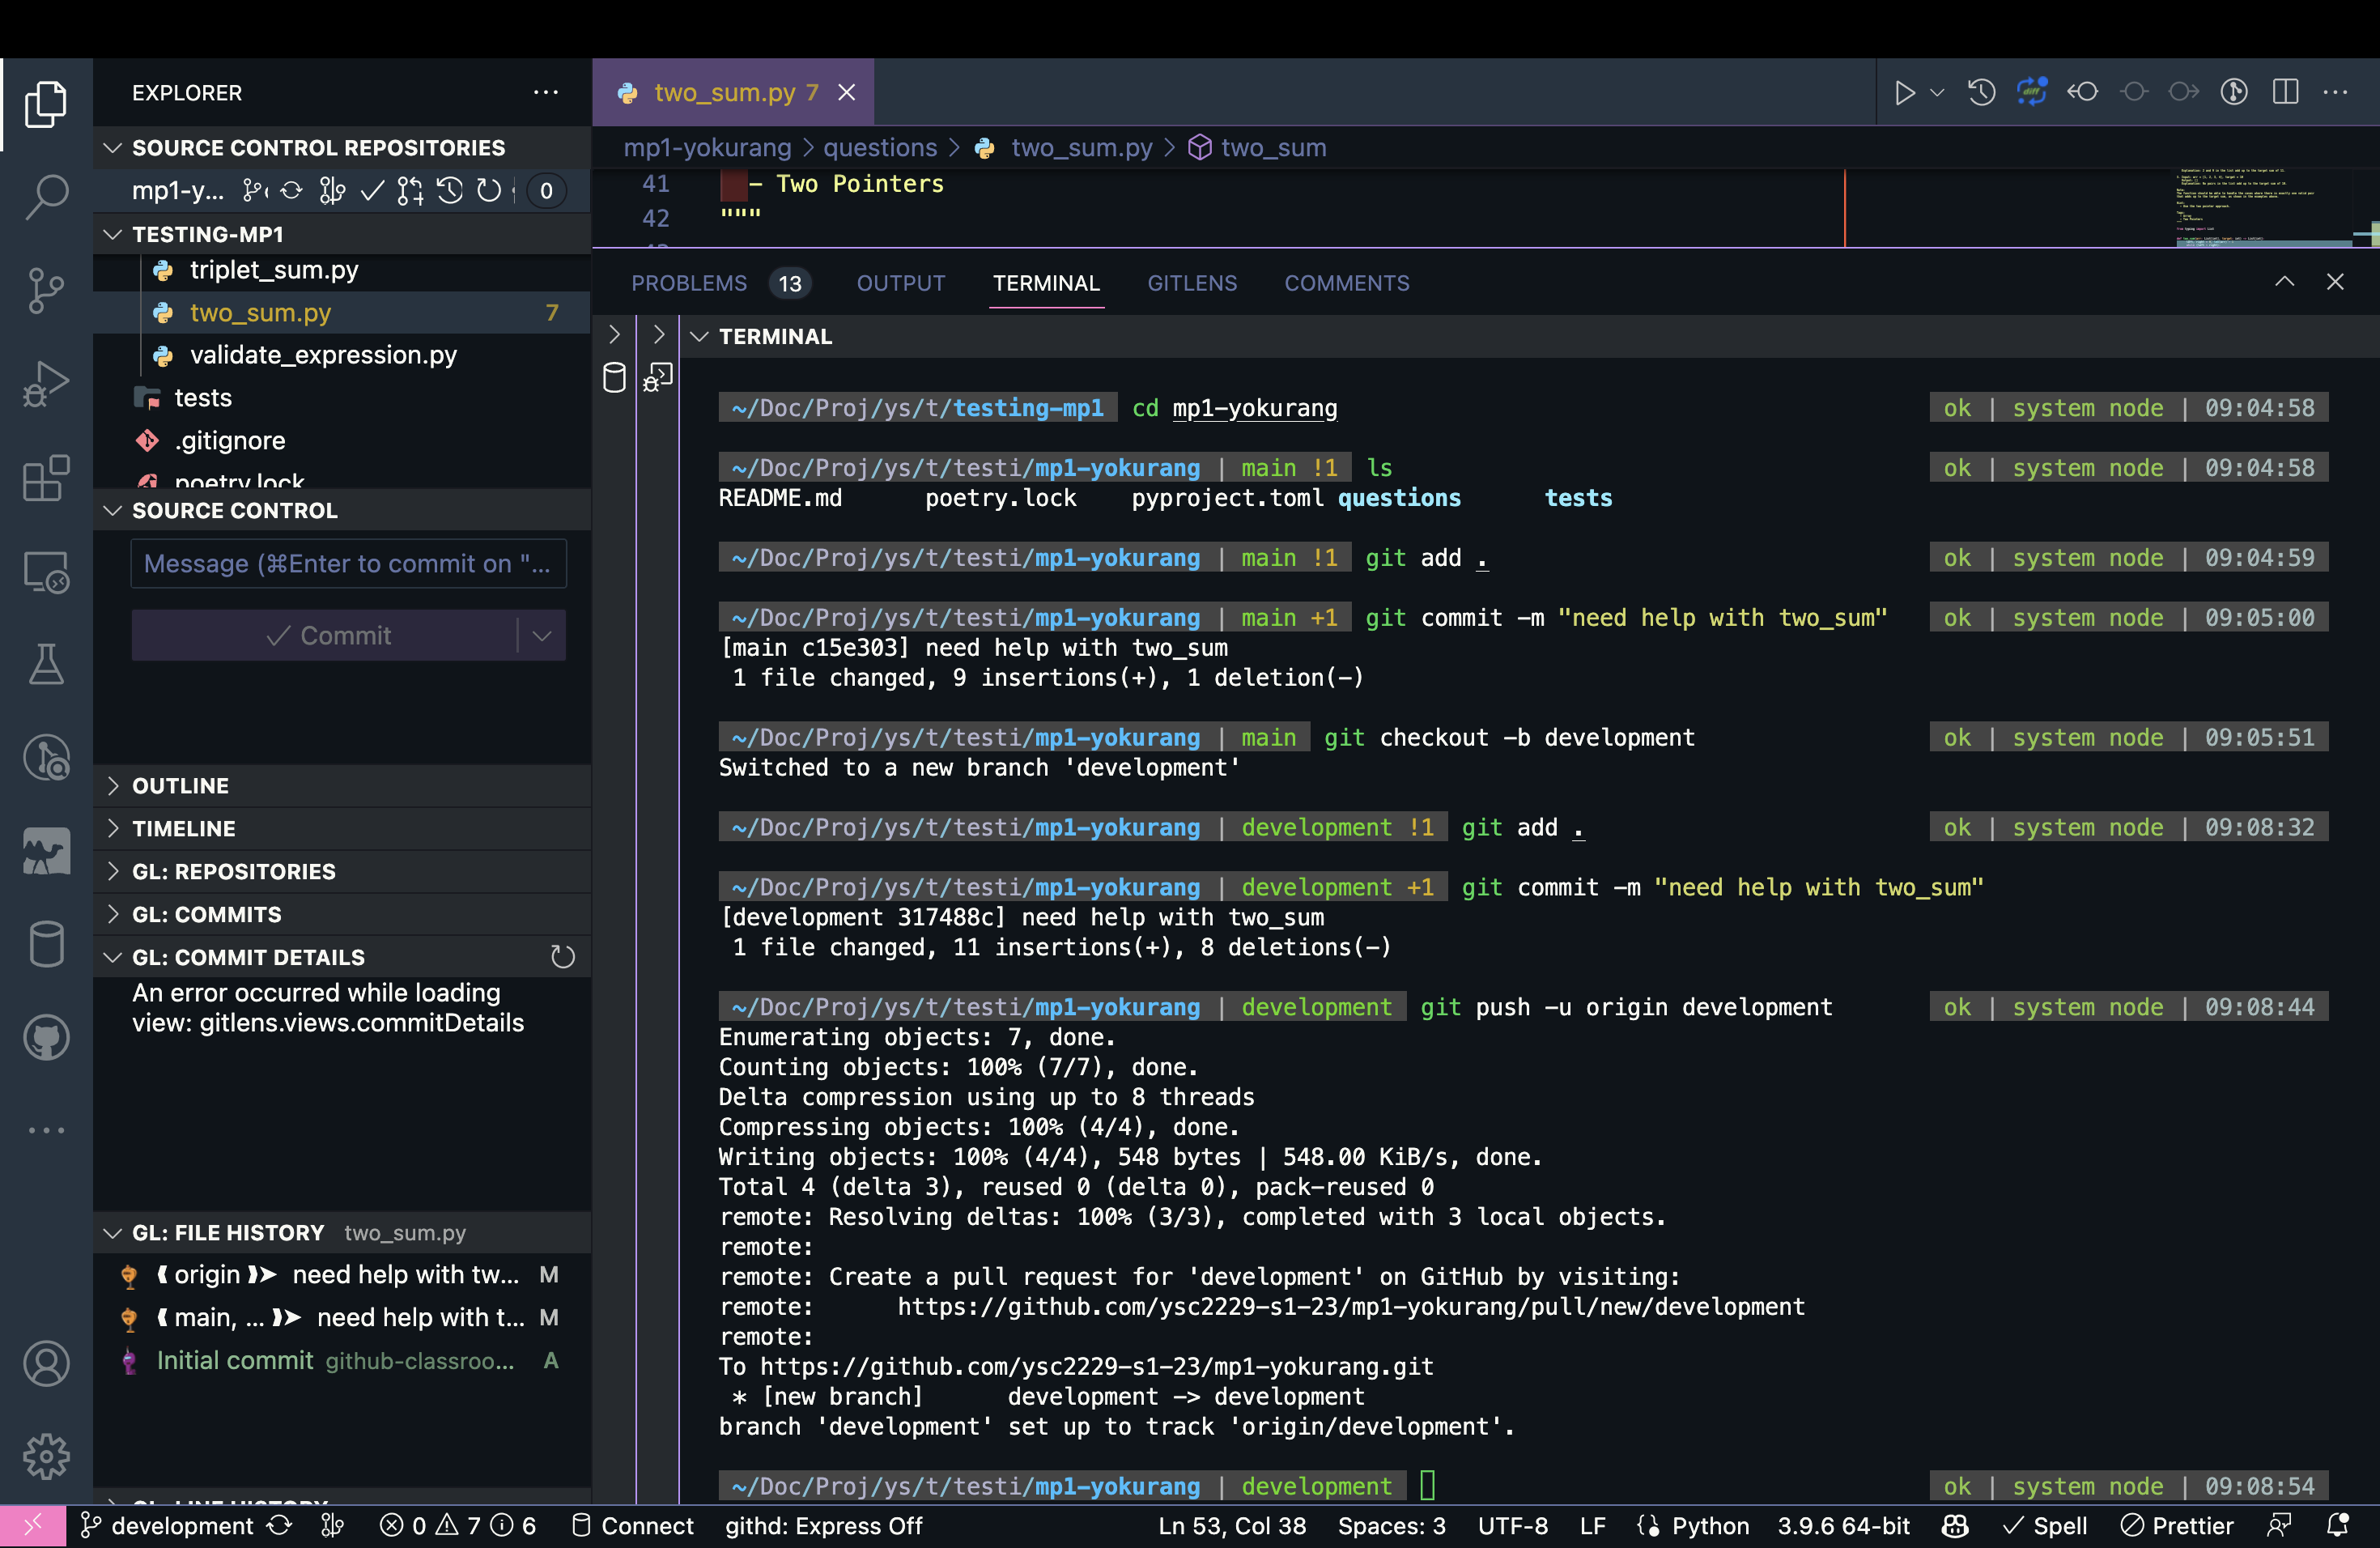
\includegraphics[width=\textwidth,height=0.4\textheight,keepaspectratio]{assets/create-a-branch-and-push.png}
\end{frame}

\begin{frame}{Open Pull Request}
    Return to your repository page to open a pull request.
    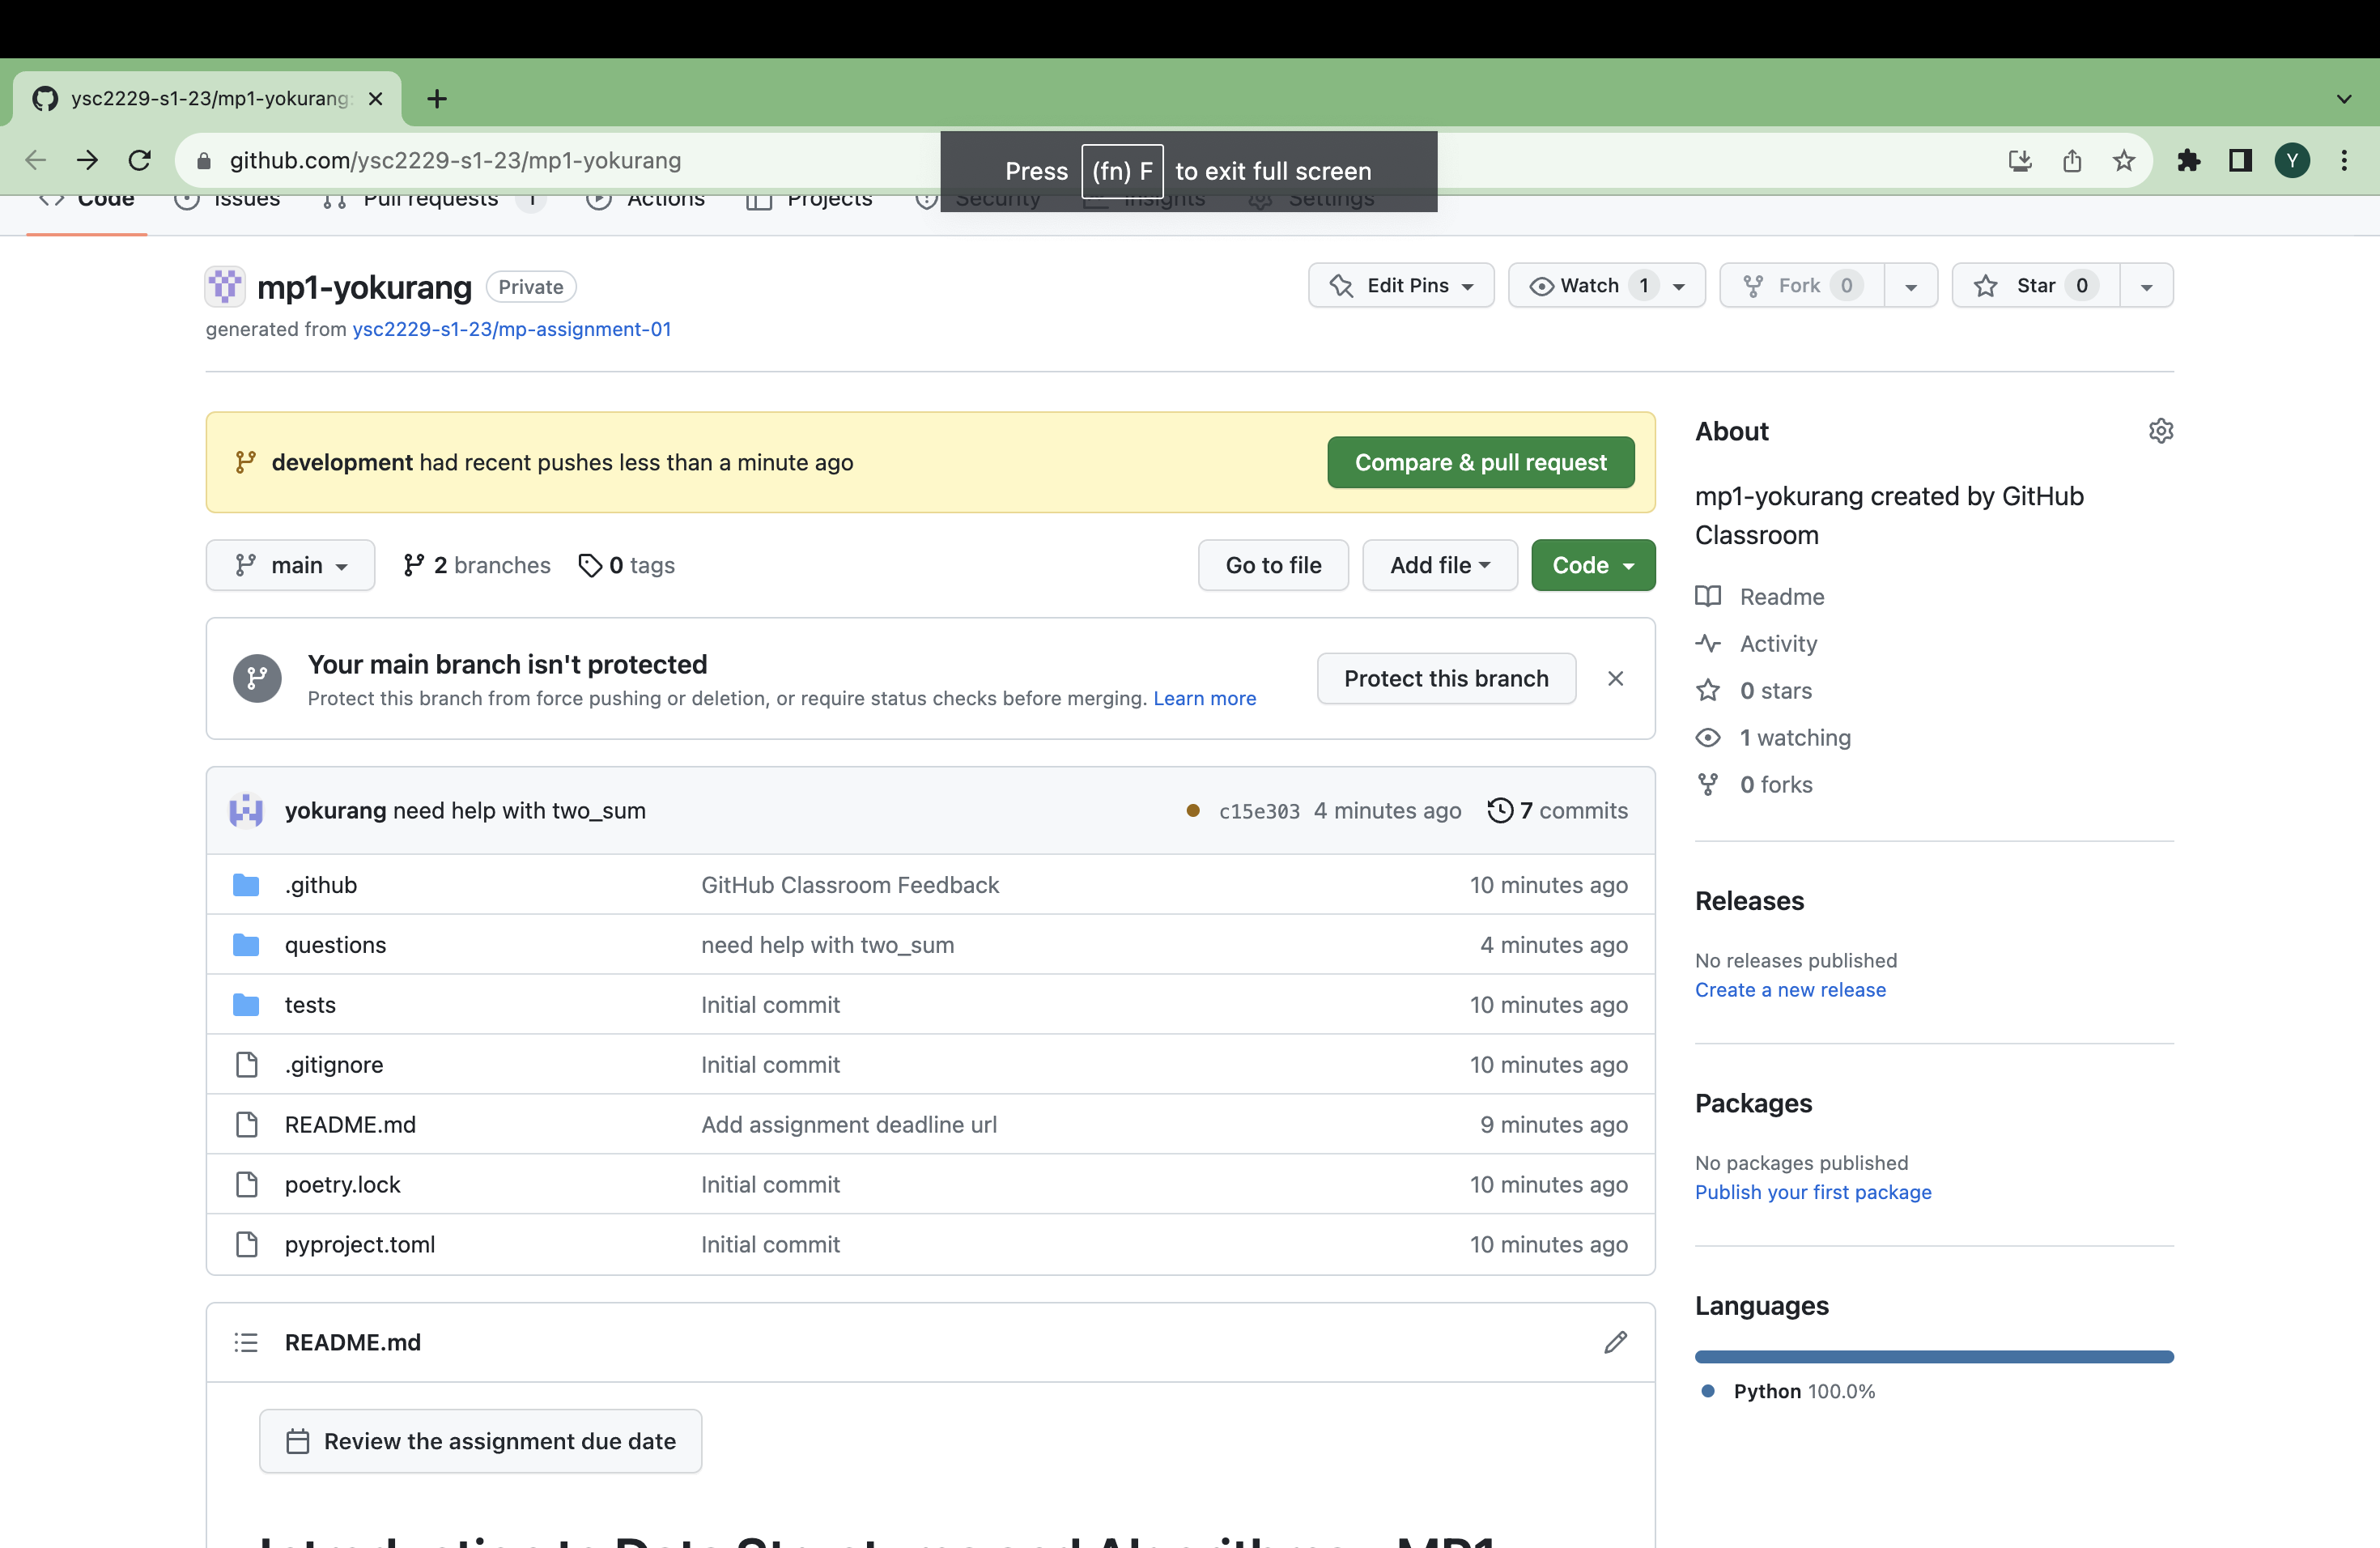
\includegraphics[width=\textwidth,height=0.7\textheight,keepaspectratio]{assets/go-to-repository-page.png}
\end{frame}

\begin{frame}{Detail Your Issue}
    Provide a clear title and description for your pull request.
    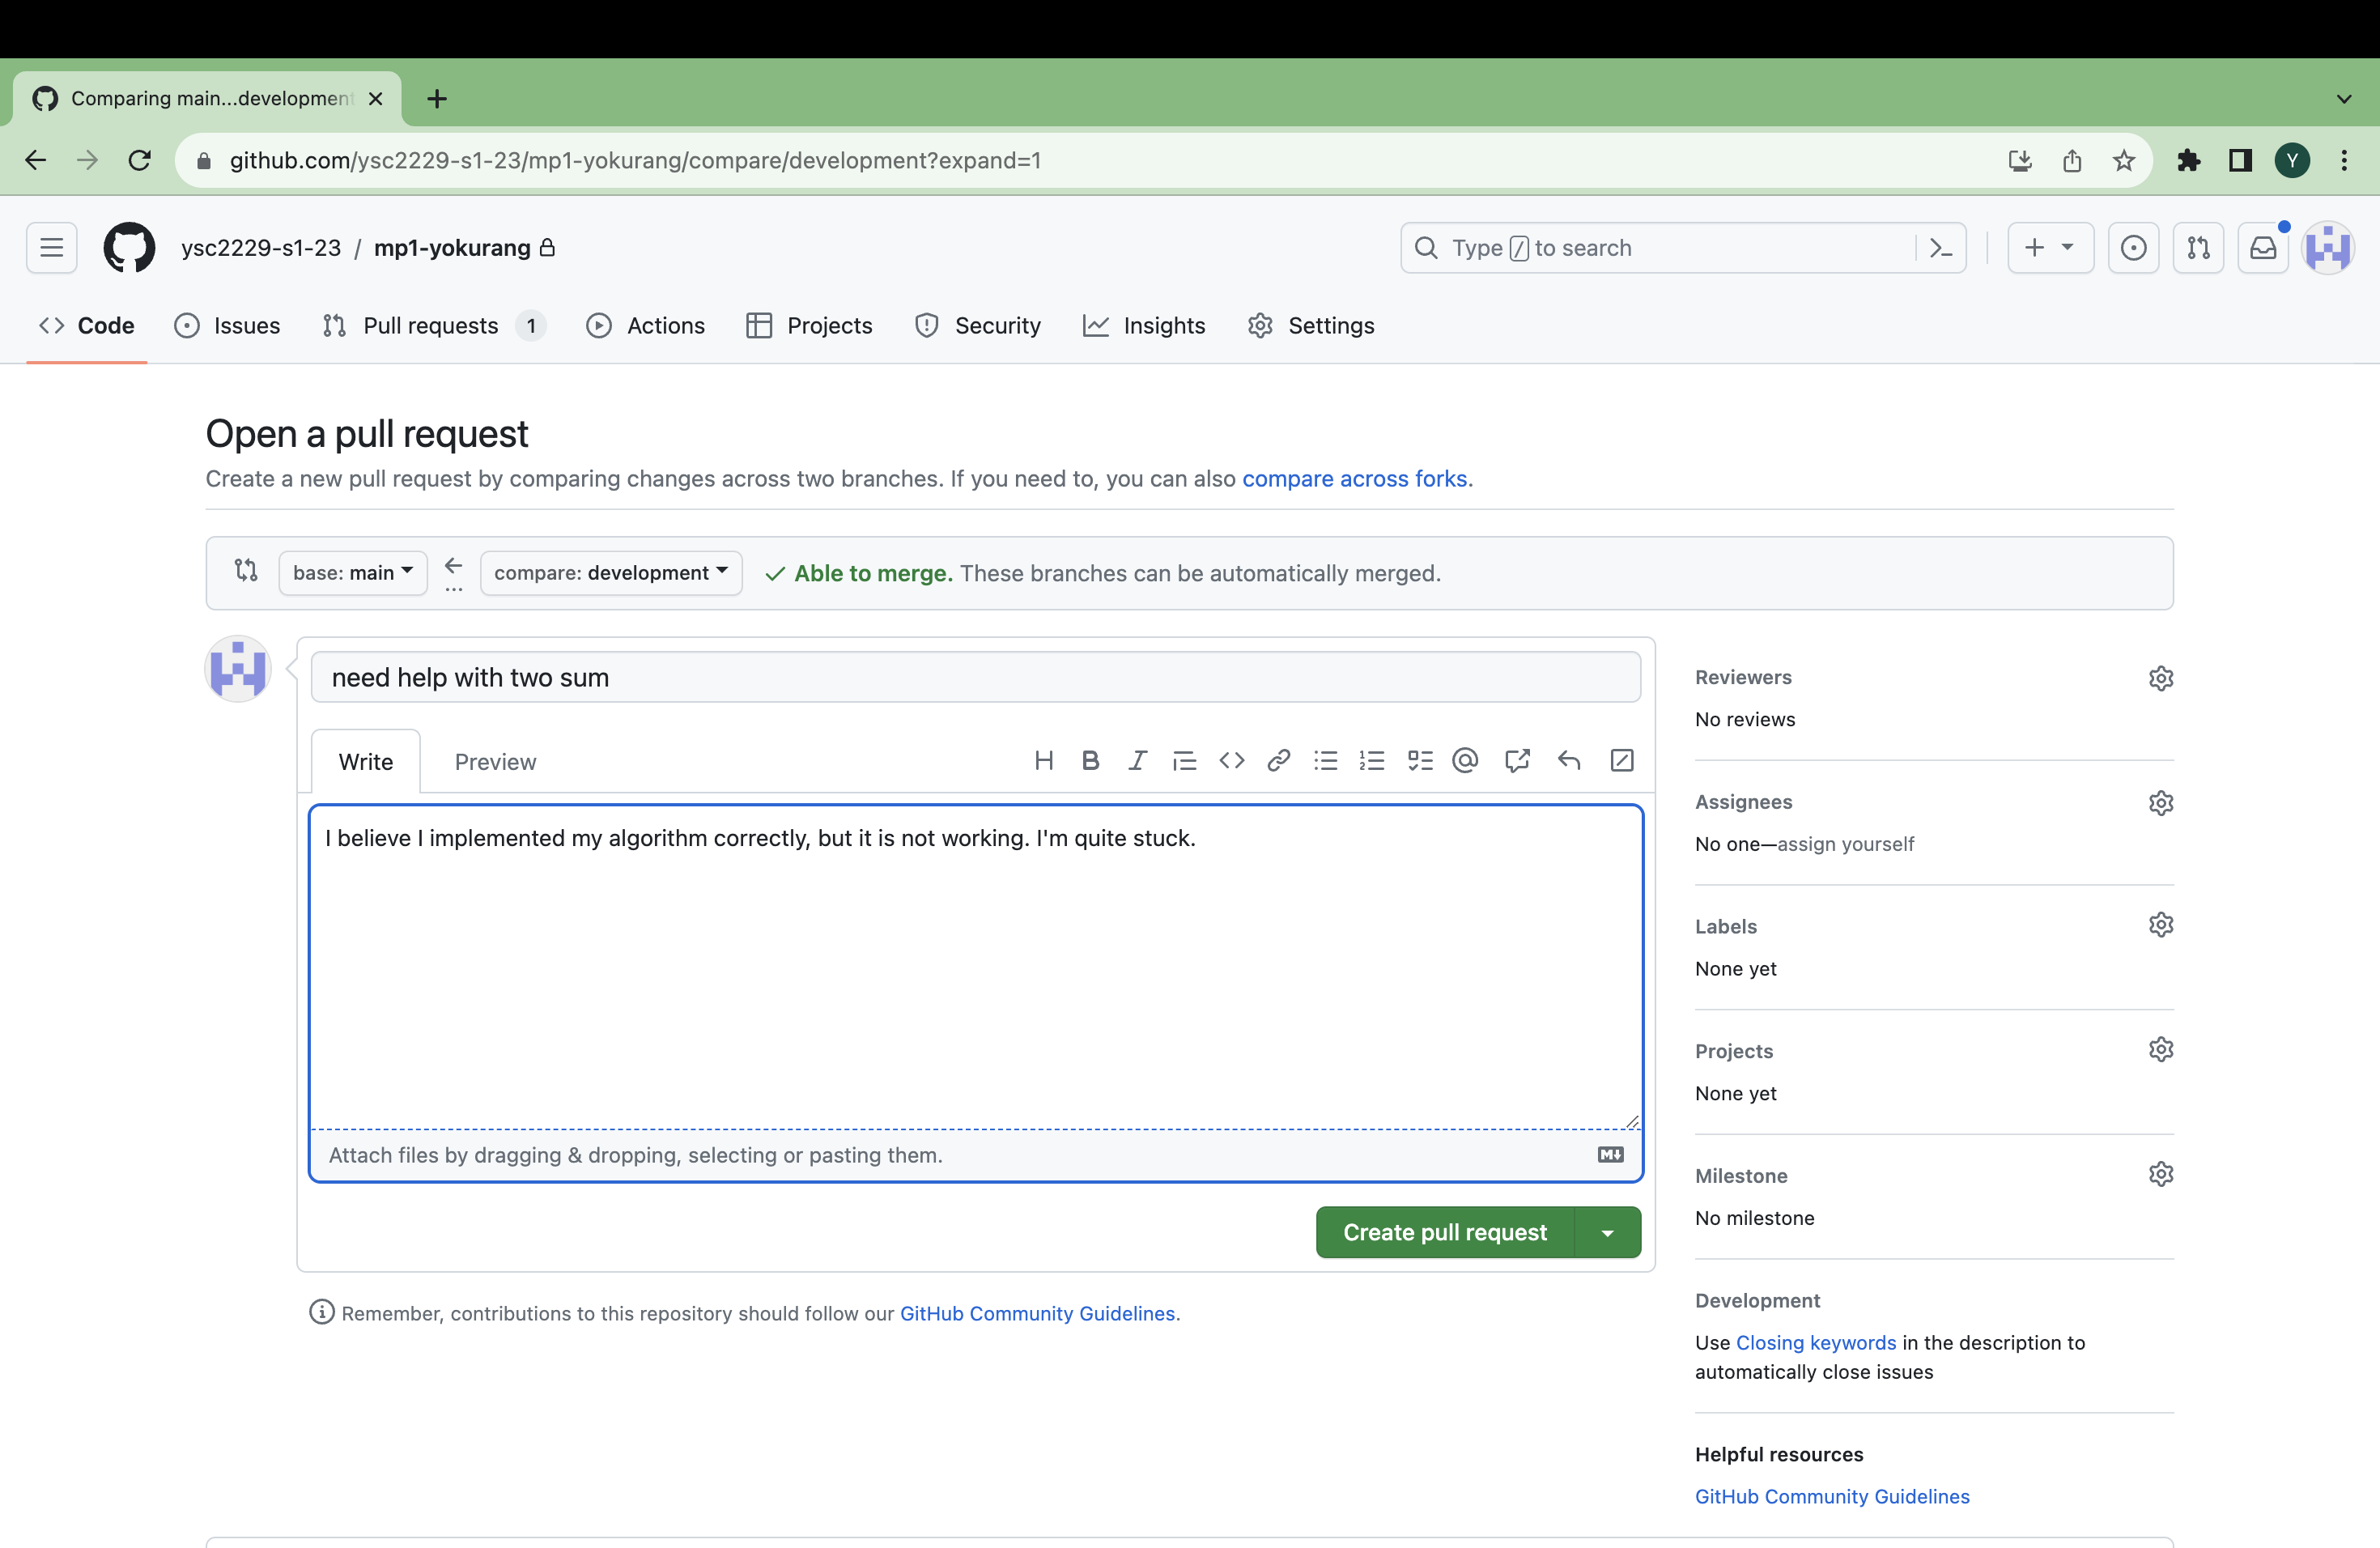
\includegraphics[width=\textwidth,height=0.7\textheight,keepaspectratio]{assets/write-some-comments-on-the-pull-request.png}
\end{frame}

\begin{frame}{Collaborative Assistance}
    Helpers can now review and comment on your code.
    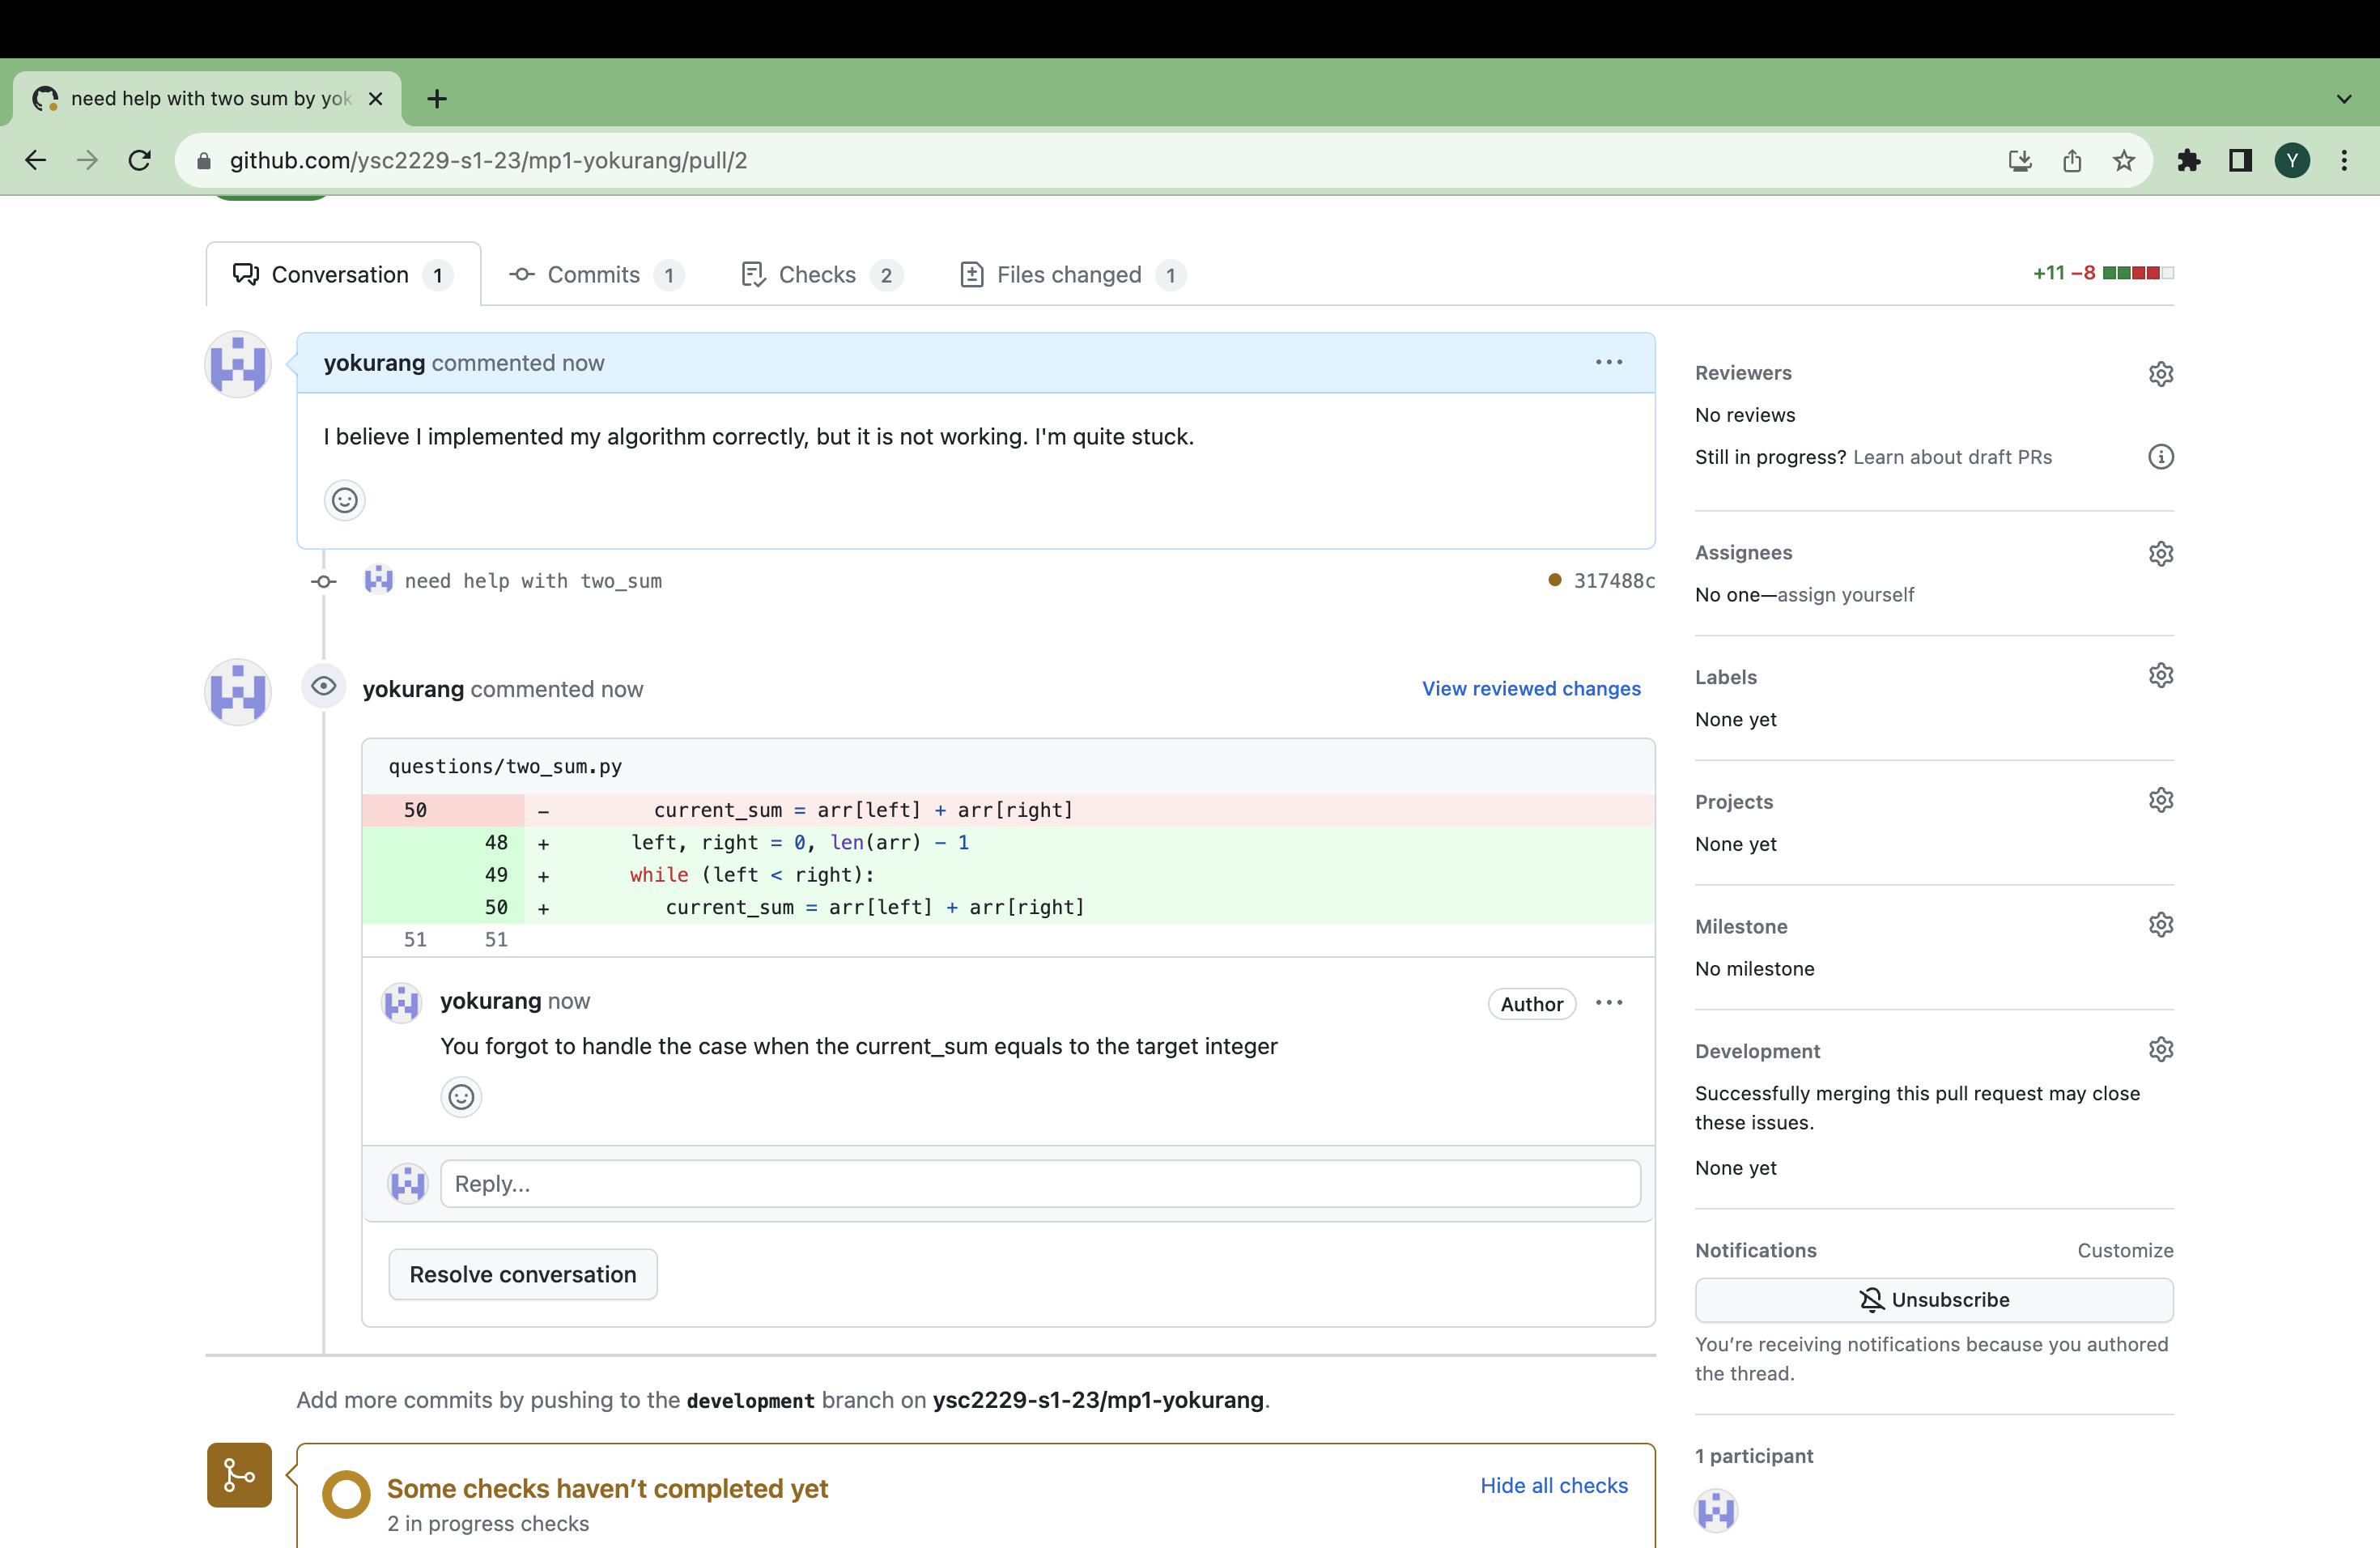
\includegraphics[width=\textwidth,height=0.7\textheight,keepaspectratio]{assets/wait-for-comments-and-check.png}
\end{frame}

\begin{frame}{VSCode: Reload Window}
    Remember to reload your window in VSCode.
    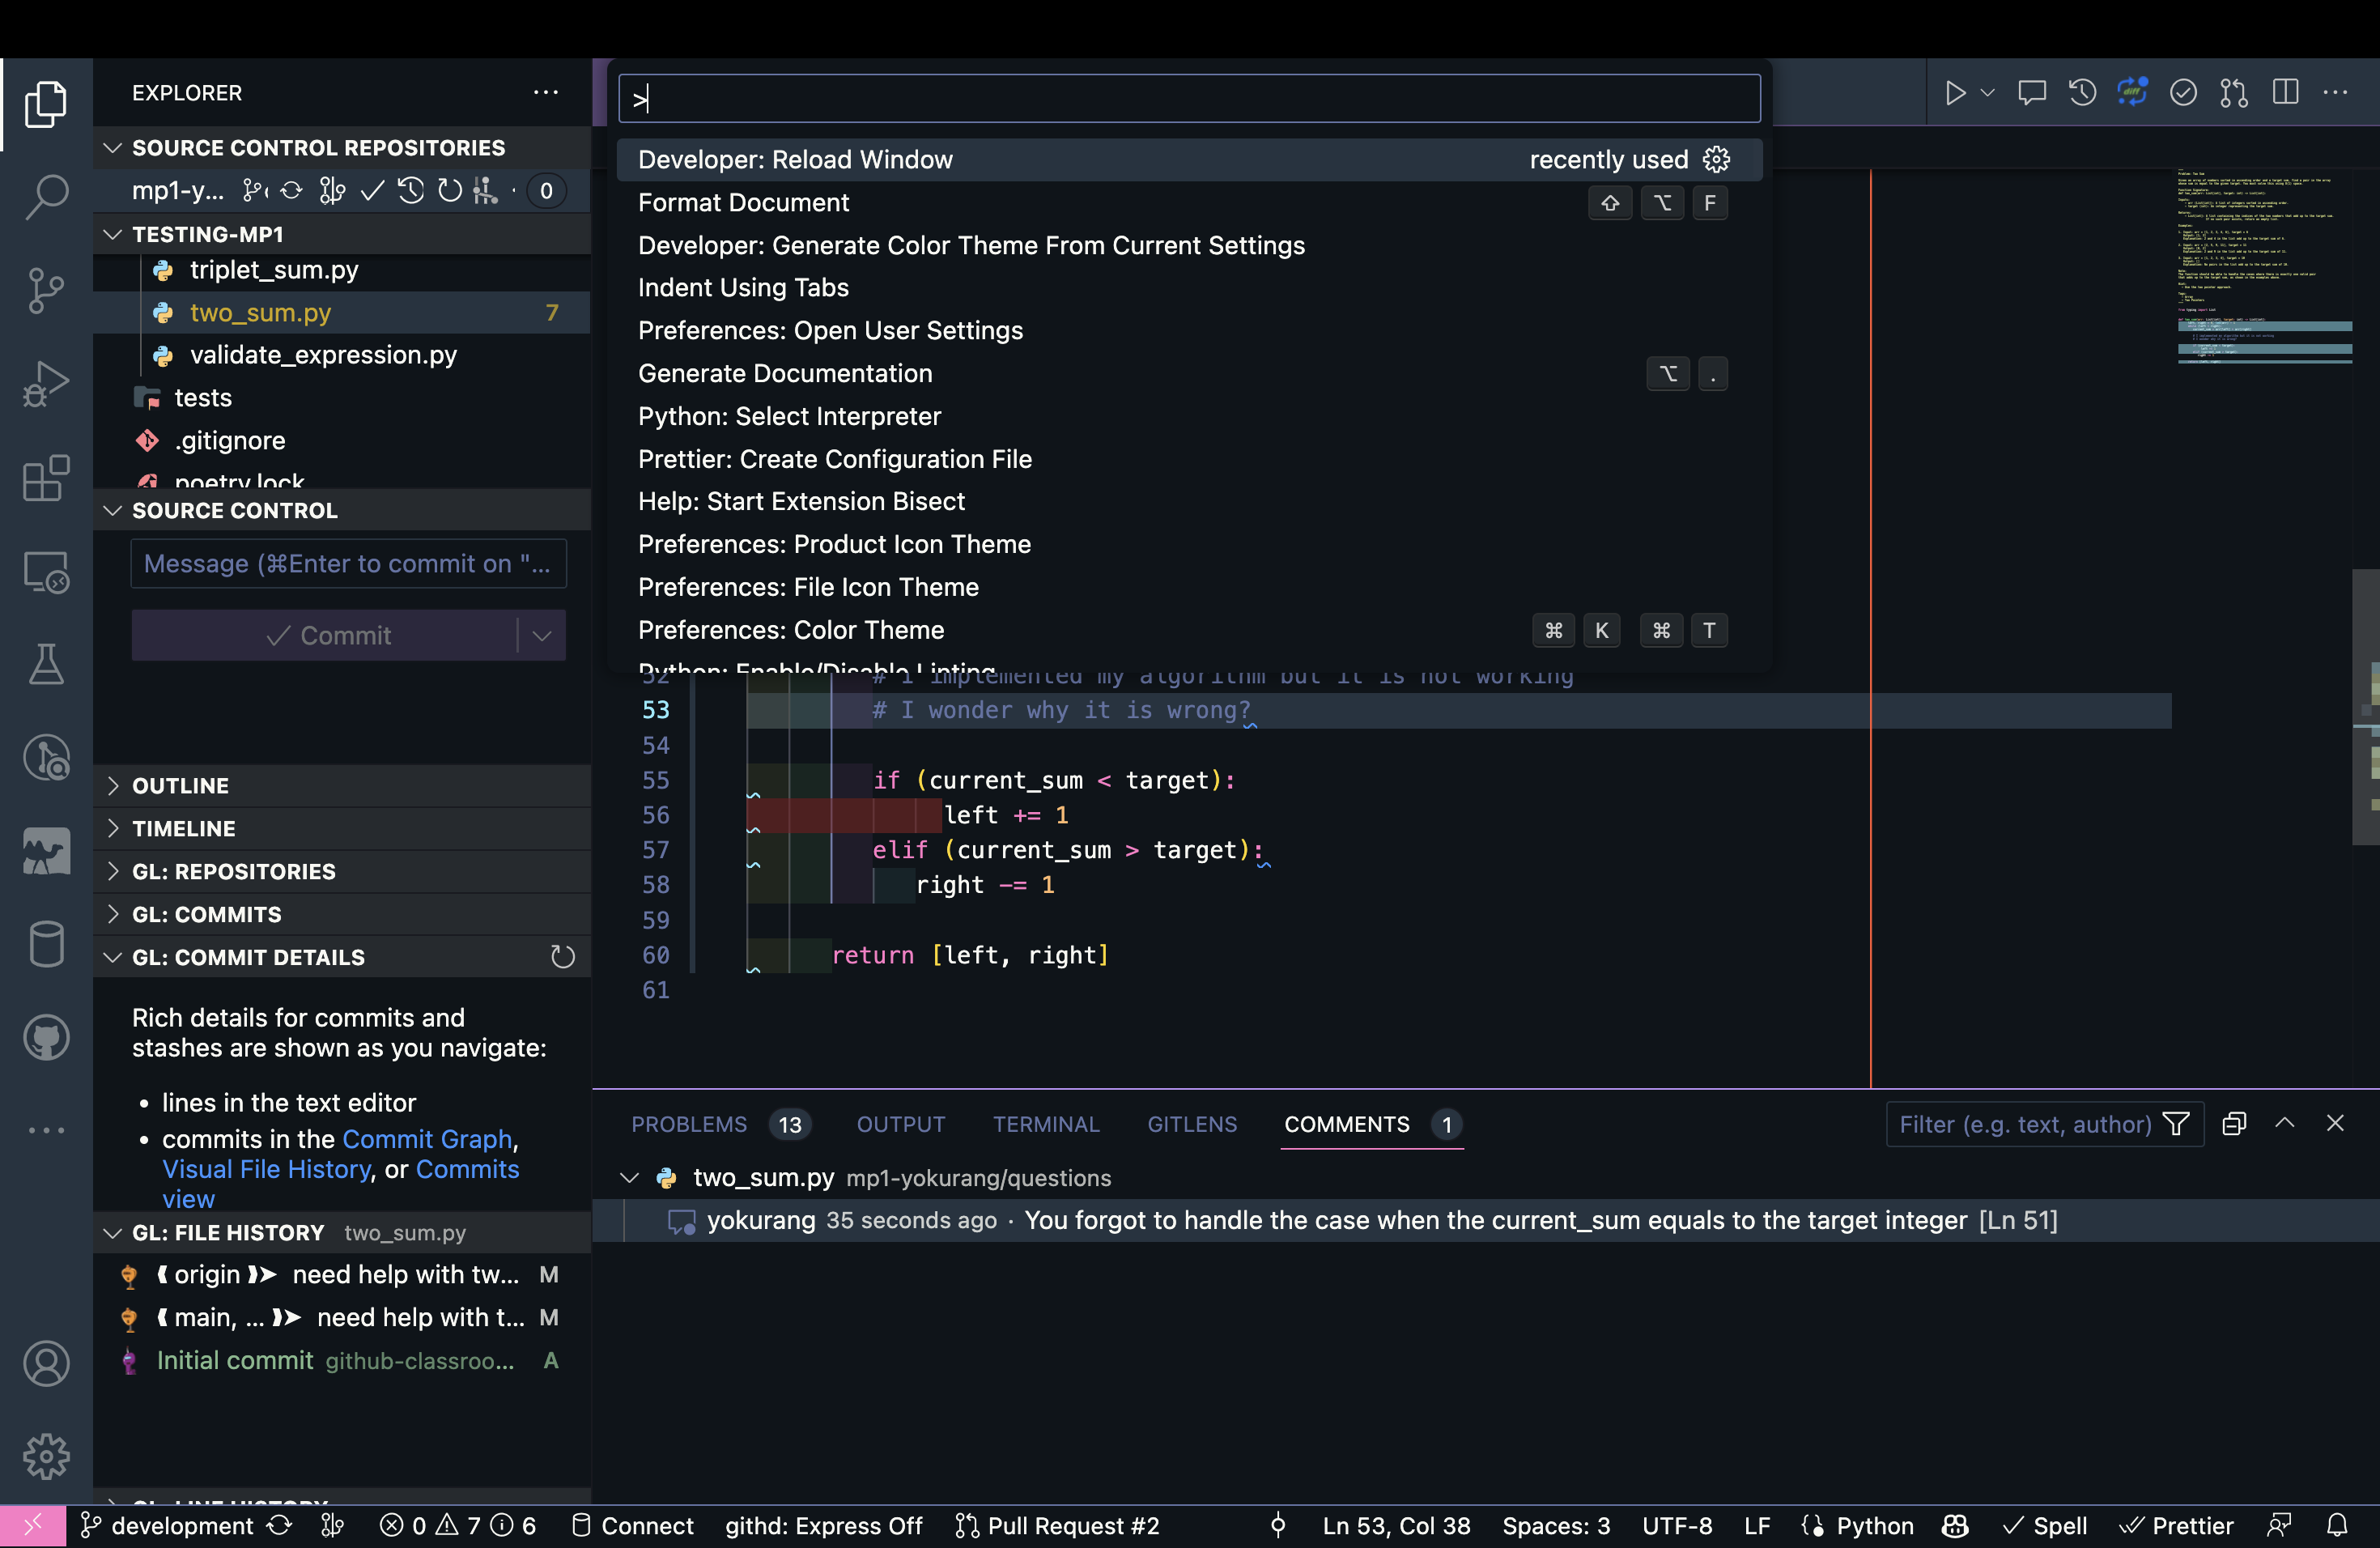
\includegraphics[width=\textwidth,height=0.7\textheight,keepaspectratio]{assets/reload-your-window.png}
\end{frame}

\begin{frame}{View Comments in VSCode}
    After reloading, observe the comments directly in your editor.
    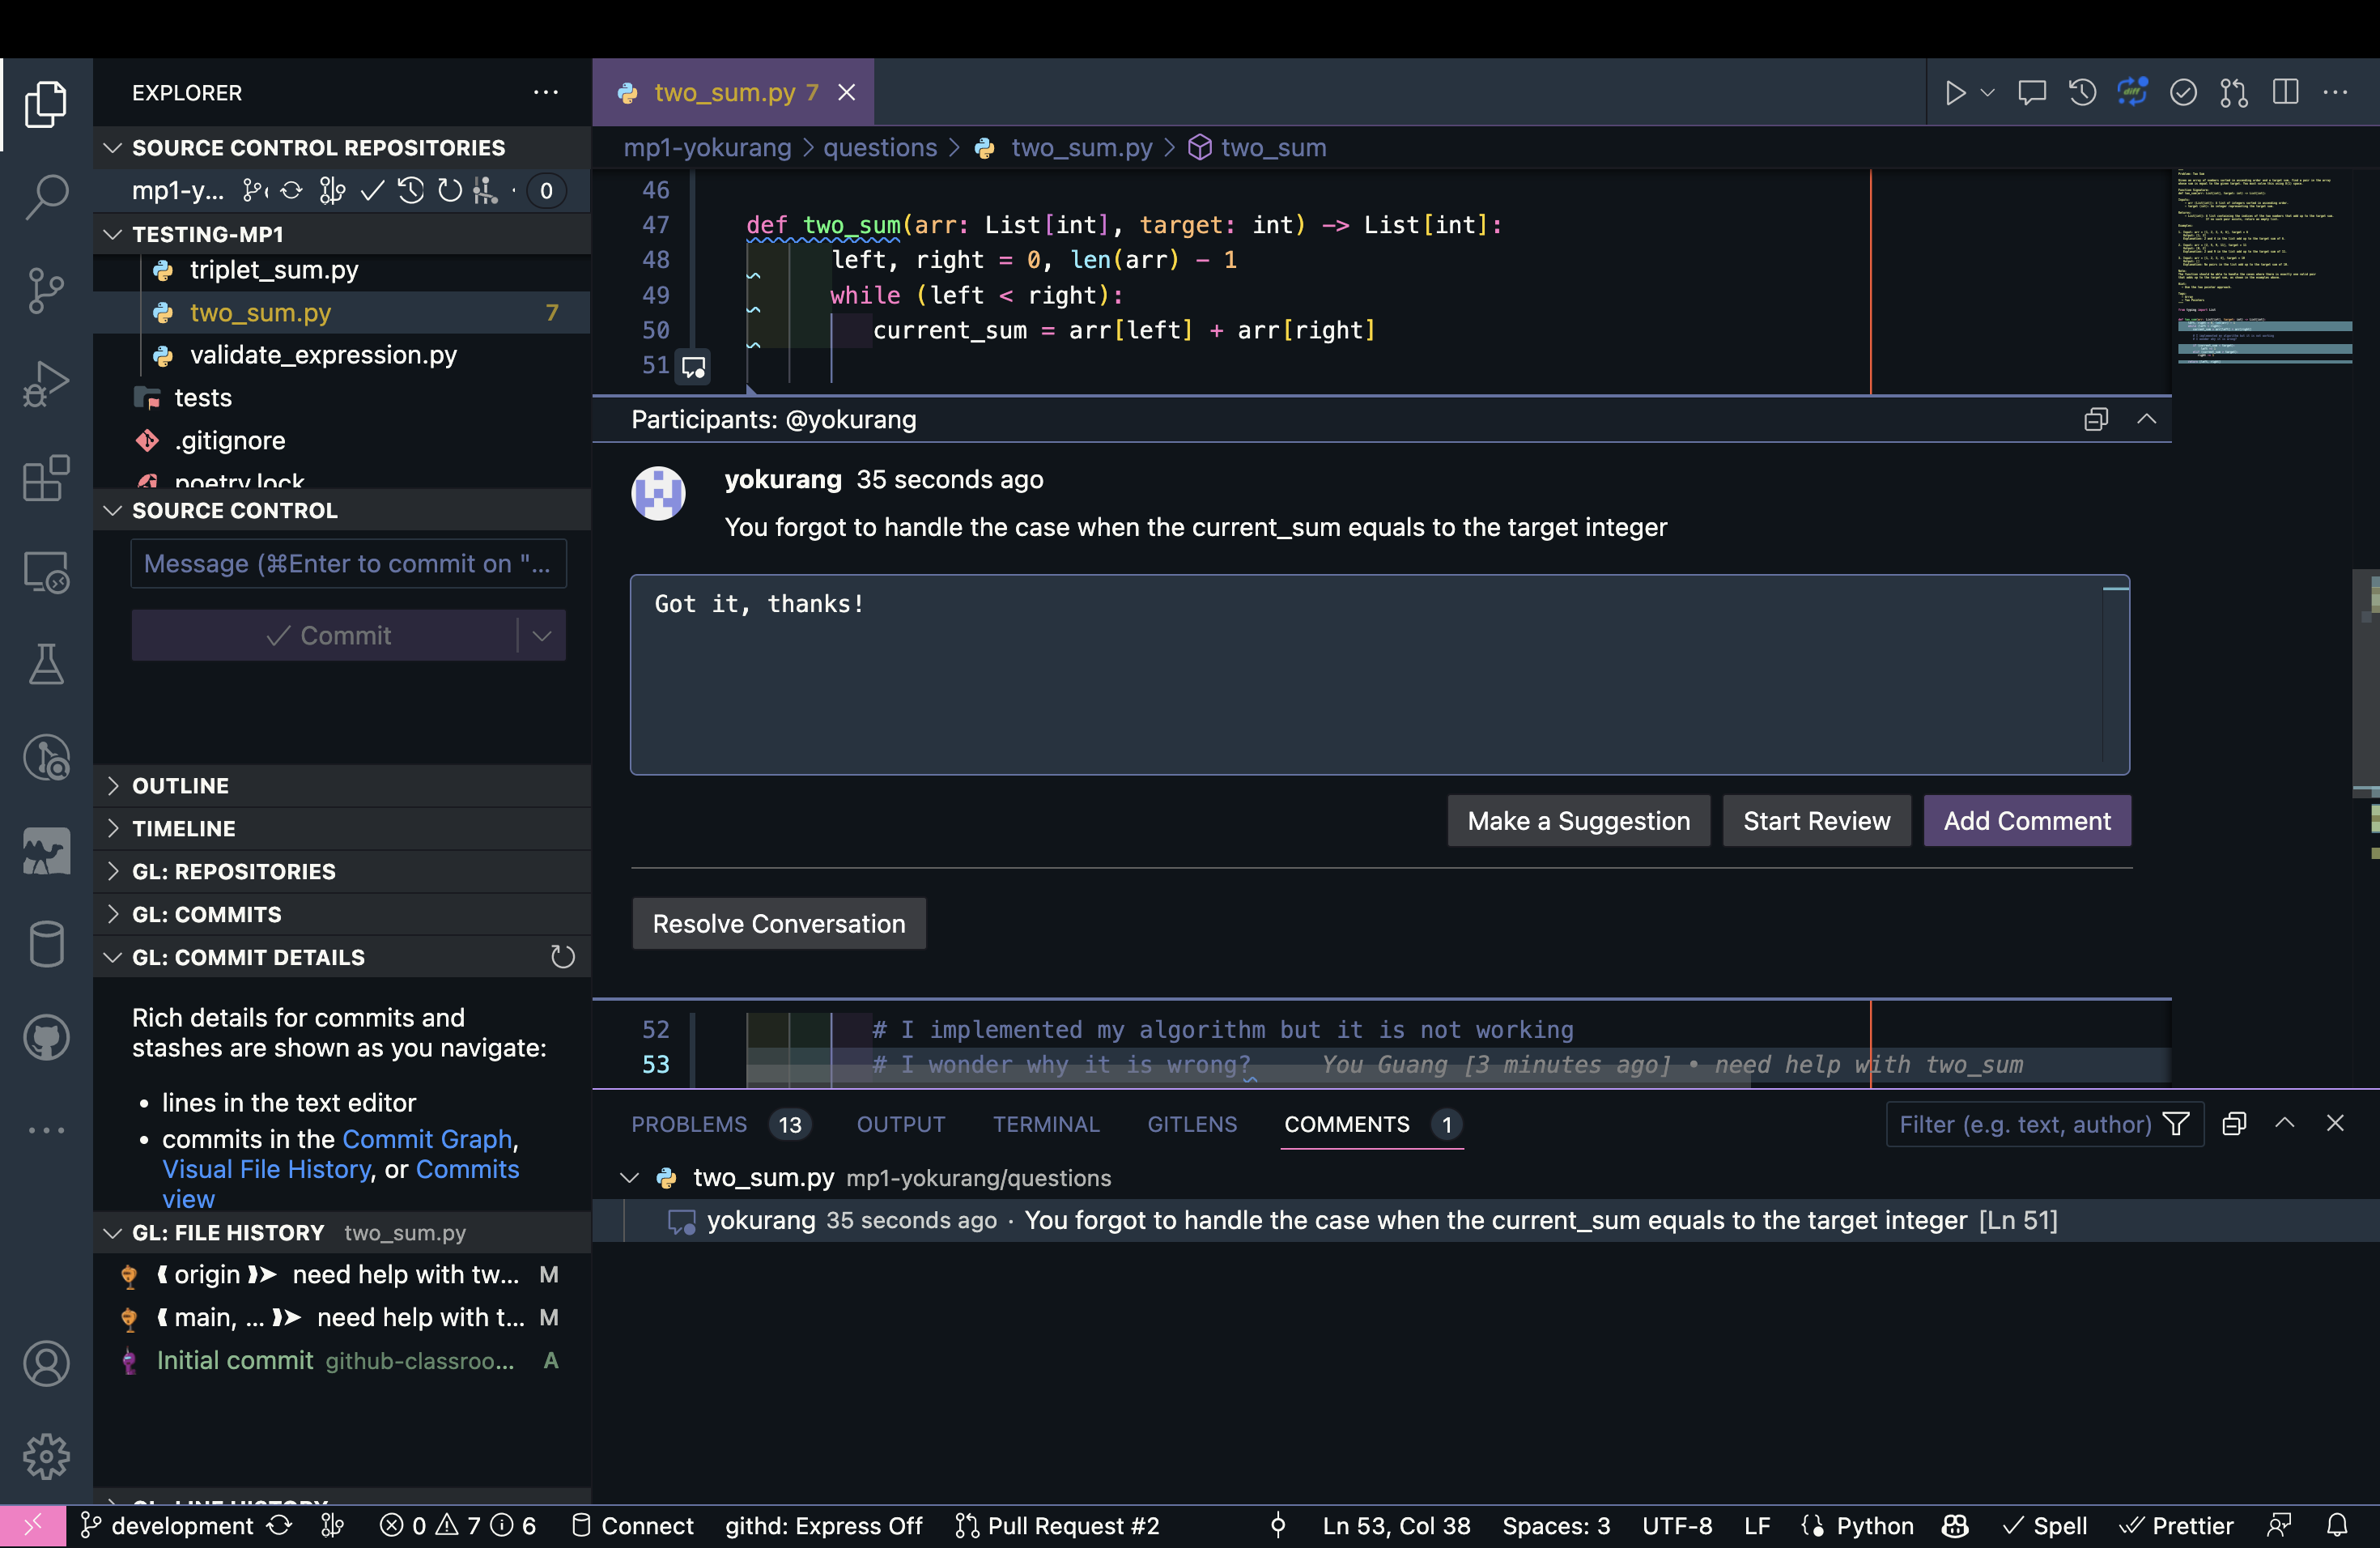
\includegraphics[width=\textwidth,height=0.7\textheight,keepaspectratio]{assets/check-comments-in-vscode.png}
\end{frame}

\begin{frame}{Merge the Pull Request}
    When resolved, merge your pull request on GitHub.
    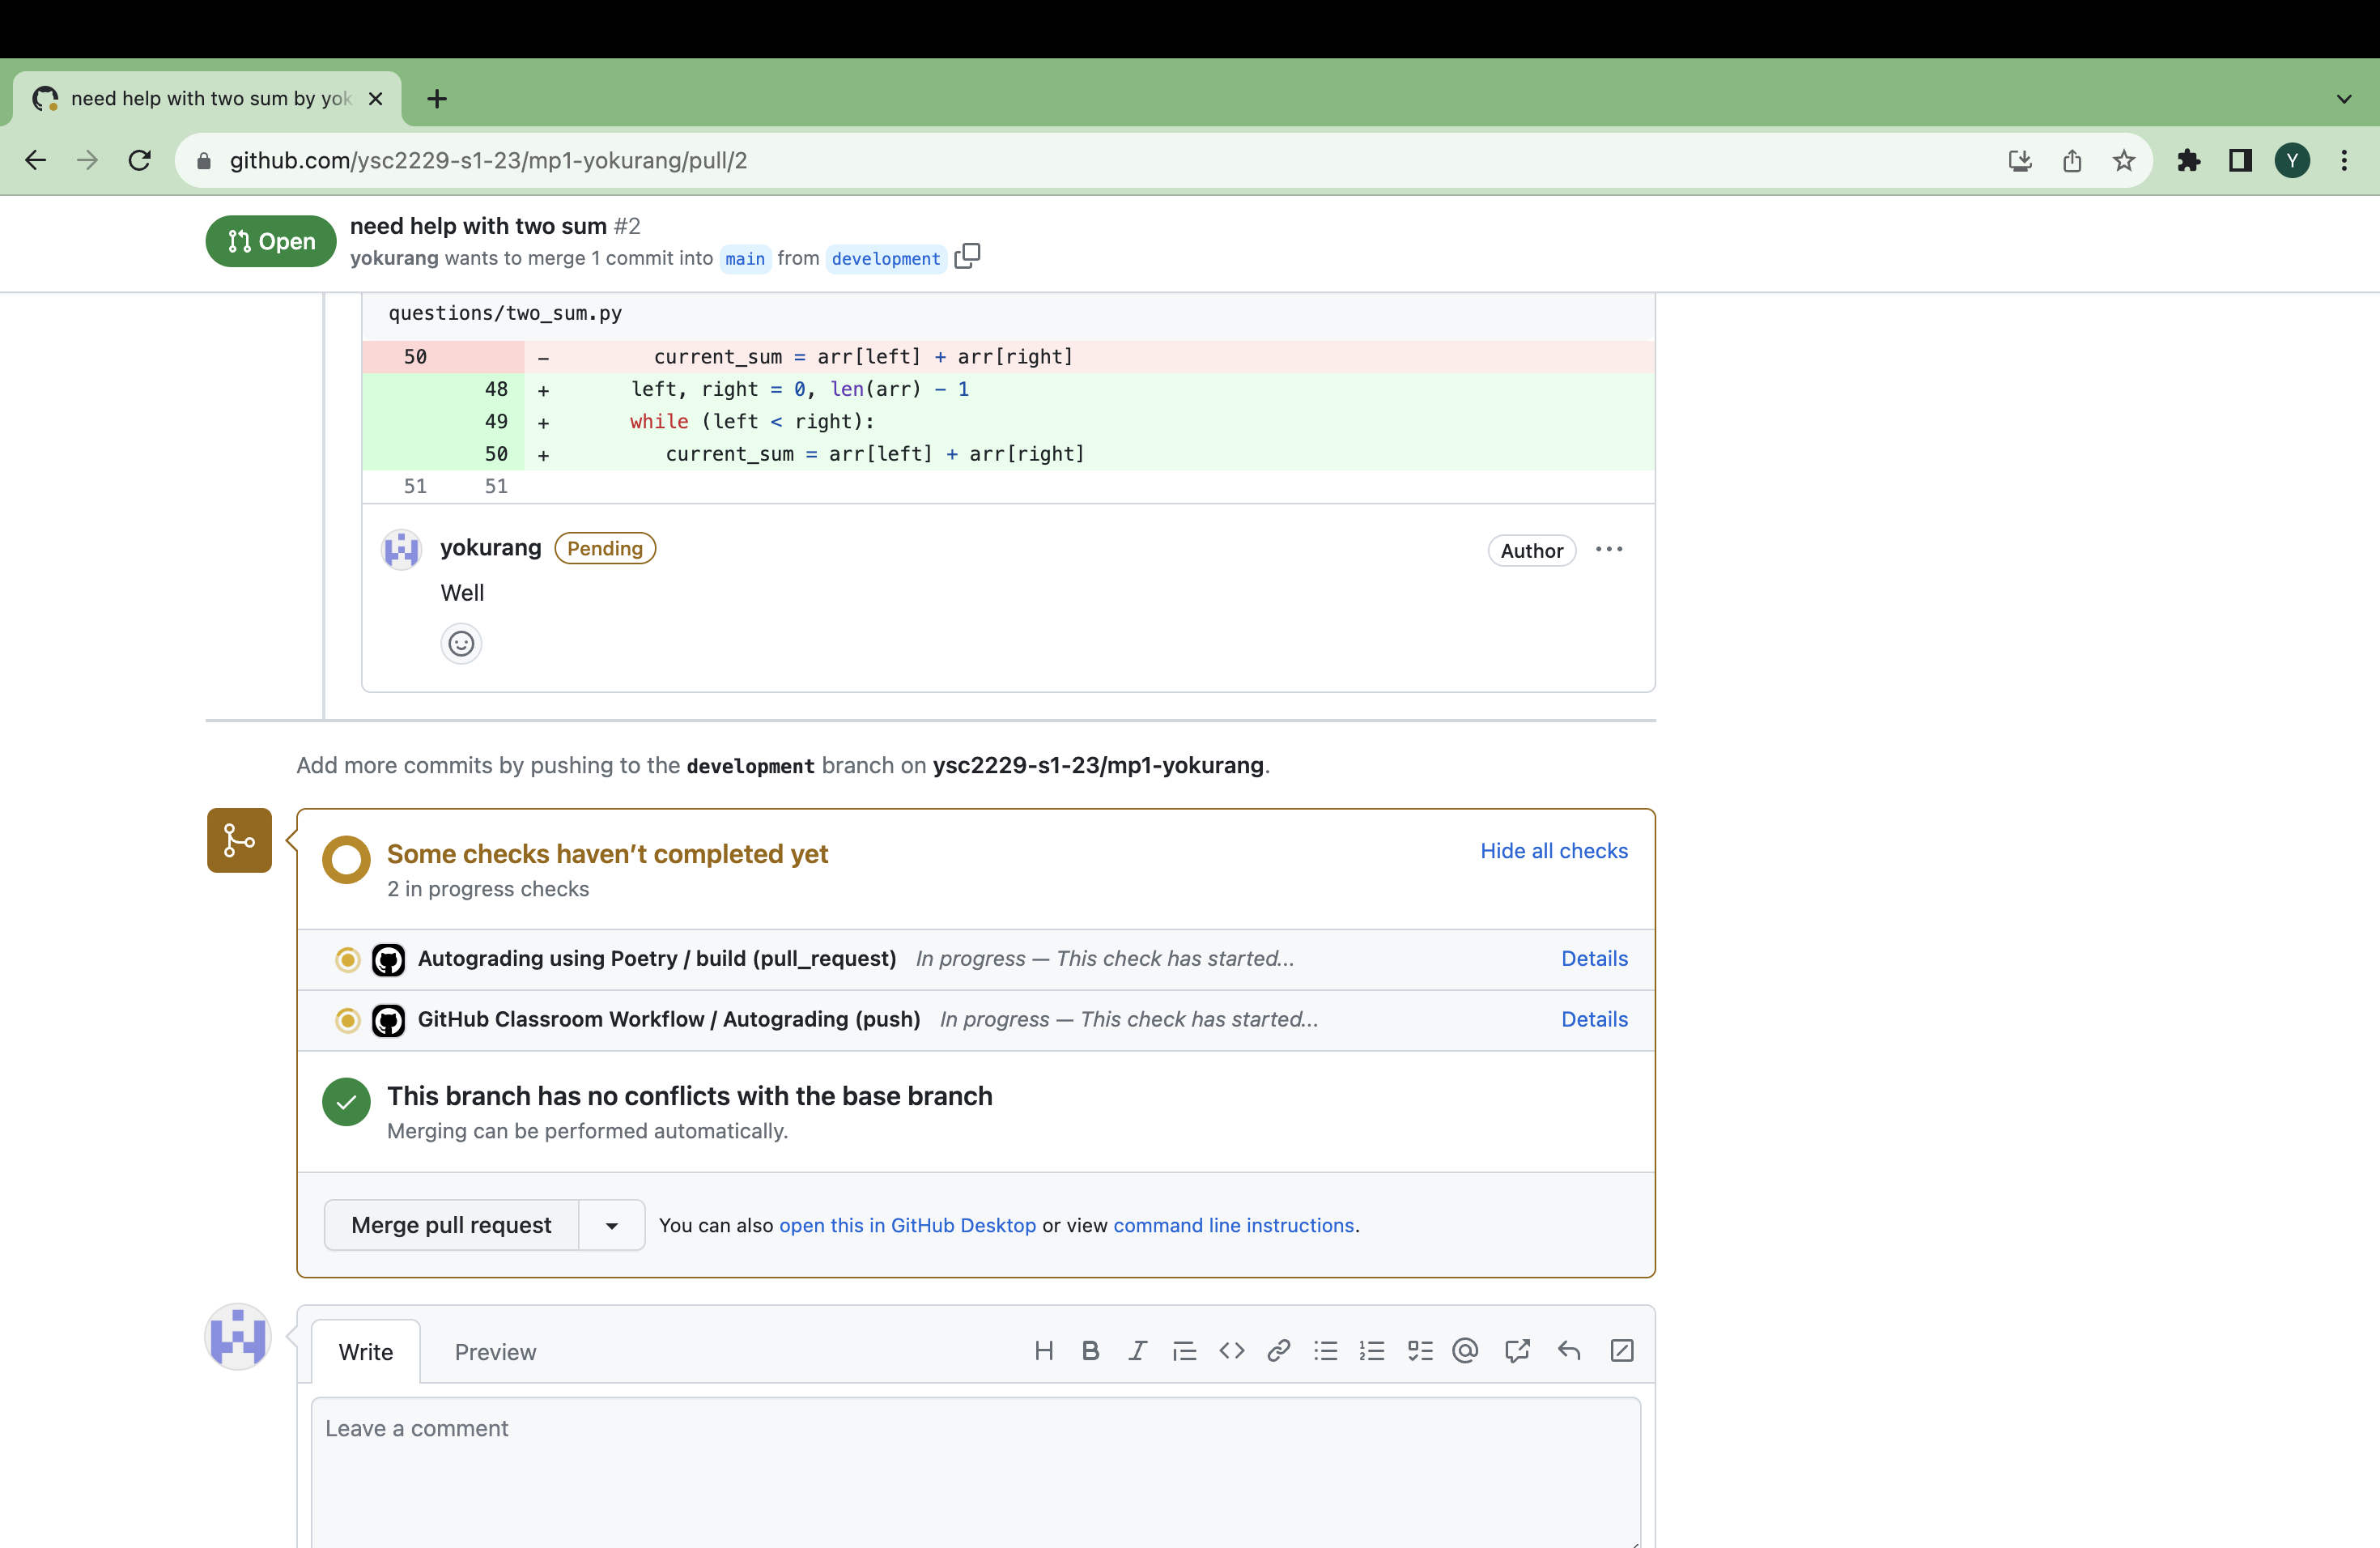
\includegraphics[width=\textwidth,height=0.7\textheight,keepaspectratio]{assets/merge-after-done.png}
\end{frame}

\begin{frame}{Grading Considerations}
    \centering
    \large Remember, only the \texttt{main} branch will be considered for grading.
\end{frame}

\end{document}
